\subsection{Versuchsaufbau}
\label{sec:Versuchsaufbau}

Die optischen Elemente, also die Lichtquelle, die Gegenstandshalterung, die Linsen und der
Schirm,
werden auf einer optischen Bank auf Reitern befestigt. An dieser Bank ist ein Lineal angebracht,
an dem die verschiedenen Abstände zueinander abgelesen werden können.
Zur Messung der Bildgrößen und Gegenstandsgrößen wird ein Lineal verwendet.
Diese Reiter ermöglichen das Verschieben dieser Elemente auf der optischen Bank.
Die Lichtquelle ist als Halogenlampe und der Gegenstand als "Perl L" realisiert.
Weiterhin werden Linsen bekannter Brennweite (hier $f=\SI{100}{\milli\meter}$ und
$f=-\SI{100}{\milli\meter}$) und eine Linse unbekannter Brennweite verwendet. \\
Die Linse unbekannter Brennweite entspricht einer mit Wasser gefüllten Linse, wobei das Wasservolumen
innerhalb dieser Linse mit Hilfe einer Spritze variiert werden kann. Aufgrund der
Dichtezunahme erhöht sich der Brechungsindex und somit die Brennweite der Linse.
Hierbei ist zu beachten, dass das Wasservolumen bei einer Messung konstant gehalten wird.

\subsubsection{Bestimmung der Brennweite einer Sammellinse durch Messung der Gegenstandsweite g und Bildweite b}
\label{sec:gundb}
Bei der Bestimmung der Brennweite einer Sammellinse durch die Messung der Gegenstandsweite $g$ und
der Bildweite $b$ werden die Halogenlampe, die Gegenstandshalterung, die betrachtete
Linse und der Schirm
in dieser Reihenfolge auf der optischen Bank auf Reitern befestigt.
Der Gegenstand - das "Perl L" - wird an der Gegenstandshalterung angebracht.

\subsubsection{Bestimmung der Brennweite einer Sammellinse nach der Methode von Bessel für
weißes, rotes und blaues Licht}
\label{sec:bessel}
Die Anordnung der optischen Elemente für die Messung nach der Methode von Bessel ist identisch
zu der Anordnung bei der Bestimmung der Brennweite über die Messung der Gegenstandsweite und der
Bildweite.
Da die chromatische Abberration untersucht werden soll, werden für die jeweiligen
Messdurchgänge ein Rot- bzw. Blaufilter vor dem Gegenstand angebracht.

\subsubsection{Bestimmung der Brennweite eines Linsensystems nach der Methode von Abbe}
\label{sec:abbe}
\begin{figure}
  \centering
  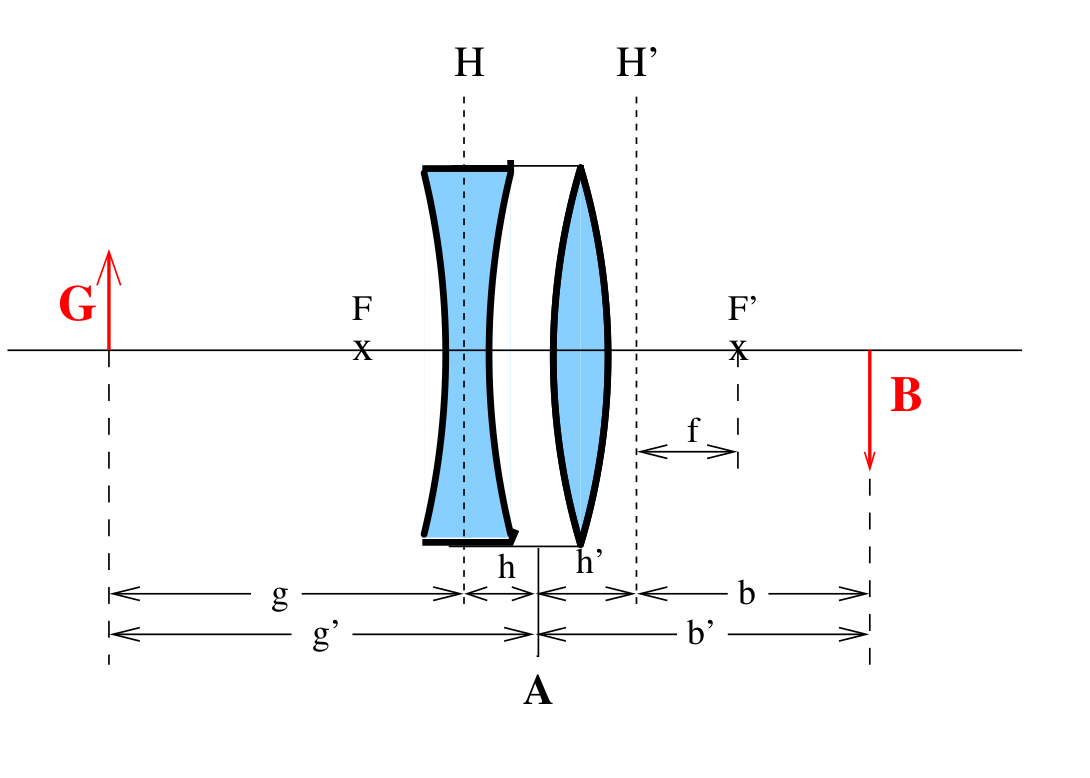
\includegraphics[width=0.6\textwidth]{Bilder/Linselol.png}
  \caption{Schematischer Aufbau des Linsensystems für die Bestimmung dessen Brennweite nach der Methode von Abbe.}
  \label{fig:lensesystemlol}
\end{figure}
Für die Bestimmung der Brennweite eines Linsensystems wird der Aufbau aus Abbildung
\ref{fig:lensesystemlol} verwendet.
Die einzige Veränderung ist also eine zusätzliche Zerstreuungslinse mit einer Brennweite von
$f_{\mathrm{Z}} = -\SI{100}{\milli\meter}$ (Sammellinse mit $f_{\mathrm{S}}=\SI{100}{\milli\meter}$).
